\section{Delayed Acoustics Model}

Investigating the physics of of a thermoacoustic interaction requires the resolving of the full nonlinear acoustics in the combustion system -- this might typically be a plenum, inlet, combustor and exhaust -- as well as the highly local reaction and diffusion phenomena located at the flame. In the case of a deflagration in a tube, the acoustics span the tube, but the premixed flame and surrounding hydrodynamics will be located only in a relatively small region of the tube. It would be natural, then, to fully resolve the flame and hydrodynamics in a simulated region and leave the acoustics which are the dominant effect upstream and downstream of the flame to be modelled separately. Assume at the simulation inflow that we can decompose the pressure and velocity fields, $\vb{u}=(u, v)$ in two-dimensions, as $u = \overline{u} + u_a$ and $p = \overline{p} + p_a$, where $\overline{(\cdot)}$ represents the non-acoustic field at the inflow and $(\cdot)_a$ represents acoustic fluctuations. Then the value of $\overline{u} \pm c$ determines the speed of acoustic waves through the tube. Under a linear assumption for these acoustics -- i.e.\ the assumption that $ρ \approx \overline{ρ}$ such that $\abs{ρ_a} \ll 1$ or equivalently that acoustics do not interact with each other -- the convection of an acoustic wave into a headwind and tailwind will roughly cancel out. This results in a representative time delay $τ$ for the acoustic wave to leave the simulation domain, travel a distance $l$ both ways up- or downstream, and reenter:
\begin{equation}
τ = \frac{l}{c + u} + \frac{l}{c - u} = \frac{2l}{c} \, \frac{1}{1 - \Ma} \approx \frac{2l}{c}
\end{equation}
since under the deflagration approximation $\Ma \ll 1$. This is the time delay we will associate with the simulation inflow and outflow. Thus, the tube length is represented by the delayed reentry of these acoustic into the inflow and outflow after a delay $τ_{\rm{U}}$ and $τ_{\rm{D}}$ respectively. This solves the linear acoustic problem in the tube upstream and downstream of the flame to leading order in Mach number. We refer to this non-DNS domain as the acoustic or fictitious domain or region.
%%%%% THIS COULD MAYBE BE CLARIFIED - FOR A GIVEN INFLOW OR OUTFLOW WITH SOUND SPEED C AND LENGTH L...
%%%%% SHOULD REALLY BRING UP HOW THE APPROXIMATIONS WE ARE MAKING ARE RELIANT ON THE LONG WAVELENGTH ASSUMPTIONS


\begin{figure}[t]
\centering
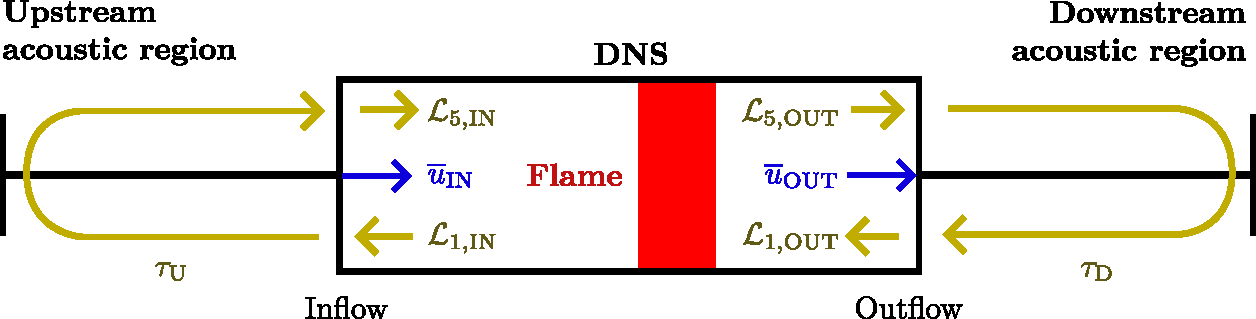
\includegraphics[scale=0.60]{assets/imgs/delay_bc_model.pdf}
\caption{A simple diagram for the simulation model.}
\label{fig:delay-model}
\end{figure}

To fit this model into the existing characteristic boundary formulation provided by NSCBC and LODI, we assume for the moment that we can store all of the outgoing acoustics as $\cl{L}_{\text{outgoing acoustic}}(t, \vb{y})$ where $\vb{y}$ parameterises the given connected inflow or outflow (this is a scalar value $y$ for two-dimensional problems with vertical inflow and outflow). For a rectangular two-dimensional horizontal tube, this becomes $\cl{L}_{1/5}(t, y)$ where the outgoing acoustic is $\cl{L}_{1}$ for left-side boundaries and $\cl{L}_{5}$ for right-side boundaries (inflows and outflows respectively in this report). A simple diagram of the acoustic behaviour is shown in \fig{fig:delay-model} as acoustic values leave and reenter the DNS domain repeatedly. Continuing with this two-dimensional example, we would impose the delayed acoustic reentry by imposing at the left-side inflow boundary that:
\begin{subequations}
\begin{equation}
\cl{L}_{5, \rm{IN}}(t, y) = \cl{L}_{5, \rm{IN}, \rm{nonreflect}}(t, y) + R_{\rm{U}} \cl{L}_{1, \rm{IN}}(t - τ, y),
\end{equation}
and at the right-side outflow boundary:
\begin{equation}
\cl{L}_{1, \rm{OUT}}(t, y) = \cl{L}_{1, \rm{OUT}, \rm{nonreflect}}(t, y) + R_{\rm{D}} \cl{L}_{5, \rm{OUT}}(t - τ, y)
\end{equation}
\end{subequations}
where $R_{\rm{U/D}}$ are the reflection coefficients at the up- and downstream acoustic boundaries. For a closed tube this would be $R = 1$ and for an open tube $R = -1$. The first terms $\cl{L}_{\dots,\: \rm{nonreflect}}$ are the required condition described in the previous chapter to stop the outgoing acoustic from being immediately reflected. Under this model, we are implicitly assuming each location at the boundary has its own one-dimensional acoustic approximation being made. For the rest of the report we instead use a simpler formulation which averages the acoustics across the boundary as they leave:
\begin{subequations}
\begin{equation} \label{eqn:L-delay-form}
\cl{L}_{5, \rm{IN}}(t, y) = \cl{L}_{5, \rm{IN}, \rm{nonreflect}}(t, y) + R_{\rm{U}} \langle \cl{L}_{1, \rm{IN}}(t - τ_{\rm{U}}, \cdot\,) \rangle_{\rm{IN}}
\end{equation}
for inflows and:
\begin{equation}
\cl{L}_{1, \rm{OUT}}(t, y) = \cl{L}_{1, \rm{OUT}, \rm{nonreflect}}(t, y) + R_{\rm{D}} \langle \cl{L}_{5, \rm{OUT}}(t - τ_{\rm{D}}, \cdot\,) \rangle_{\rm{OUT}}
\end{equation}
\end{subequations}
%(NOT SURE WHAT TO DO IF THESE WAVES DO NOT FULLY REFLECT?)
for outflows. The operator $\langle\,\cdot\,\rangle_{\rm{IN/OUT}}$ represents averaging over inflow or outflow boundary values respectively. To simplify notation, we write $\overline{\cl{L}}_{\rm{IN/OUT}}(t') \equiv \langle \cl{L}_{1/5, \rm{IN/OUT}}(t', \cdot\,) \rangle_{\rm{IN/OUT}}$ from now on. This corresponds to a single one-dimensional approximation being made for each boundary, which is of course only valid for `thin-enough' computational domains.

Since we are modelling the reaction Navier-Stokes equations, we must also impose that all other incoming $\cl{L}$ values vanish at the inflow so that no entropy, shear or mass waves enter the domain. Note that now no relaxation terms are used on either boundary -- this marks the main difference between ADCBC and NSCBC. All that is left is to apply the diffusive BCs as the remaining physical BCs. Nothing here changes with \cite{sutherland2003ImprovedBoundaryConditions}, where they use the zero normal flux conditions \equ{eqn:znf}. A further consideration to make is what happens when the acoustic field is strong enough that $\abs{\overline{u}} < \abs{u_a}$ at the inflow or outflow. Usually we expect this to happen at the inflow first since $\abs{\overline{u}_{\rm{IN}}} > \abs{\overline{u}_{\rm{OUT}}}$, i.e.\ the acoustic field has become large enough that the inflow has become an outflow at the left side of the domain. To account for this, we simply check if the sign of $\vb{u}\cdot\uvec{n}$ at this boundary where $\uvec{n}$ is the outward pointing normal and apply the conditions for $\cl{L}_m$ and diffusion correspondingly.

Relaxation terms are traditionally used under the NSCBC formulation to ensure the dependent variables -- inflow velocities, temperature or density and mass fractions and especially outflow pressure -- do not drift as characteristic waves leave the domain, not to return under perfectly non-reflecting conditions. Given that the acoustic waves will be returning under ADCBC, we do not need these relaxation terms for inflow normal velocity ($u$ in our vertical boundaries) or outflow pressure as they are closed by the full reflection of these acoustic waves. Note that if relaxation terms were imposed on top of the delayed reflections, we would be applying a further condition to a problem which is already well-posed. Note that we must have $\abs{R} = 1$ since we do not yet know how to deal with the resulting pressure drift when $\abs{R} < 1$ without using these relaxation terms. For the other variables, relaxation terms may be kept, but we have chosen to remove them under the assumption that the simulation is strongly one-dimensional and inert at the boundary. That is, no significant shear, entropy or mass waves should be leaving these boundaries, so the related dependent variables $v$, $T$, $Y_α$ will not drift.

Later on, these definitions for $\cl{L}_{1/5}$ can be extended to include an imposed acoustic field if that is desirable, e.g.\ to simulate a secondary thermoacoustic instability response. Furthermore, this method could also be extended to arbitrary numbers of delay boundaries with any boundary normal, although modelling a physical geometry in this way would be a challenge which is not explored in this work.

To summarise the method once more, we will be introducing a delay for acoustics leaving the simulation domain to model an extended acoustic domain which is not a part of this acoustic region. This will be done using non-reflecting characteristic boundaries and storing the acoustics which leave the domain. These acoustics are then simply reintroduced after the relevant time delay. We refer to these boundary conditions as \emph{Acoustic Delay Characteristic Boundary Conditions} (ADCBC).




\section{Implementing the Model}

The SUNSET code, like other CFD codes, uses a discretised temporal domain to integrate forward in time. Hence, we already only have access to the outgoing characteristics at discrete time steps and cannot recover the exact value of $\overline{\cl{L}}(t - τ)$ when $t - τ$ does not lie on a previous time step -- subscripting is omitted for now for brevity. On top of this, the step size taken by a typical combustion simulation is likely to oversample the acoustic field at the boundary, resulting in a much higher memory footprint that is required by the method. This, along with the variable time steps used in the SUNSET code means we aim for a sample rate $δt_{\rm{sample}} > δt > 0$ for these $\overline{\cl{L}}$ values. We refer to the sample times and acoustics as $\{(t_s, \overline{\cl{L}}_{s})\}_{s=1}^{N_{\rm{samp}}}$ where $s\in\bb{Z}$ enumerates these sample times so $t_{N_{\rm{samp}}}$ is the most recent sample time and $\overline{\cl{L}}_{s} \equiv \overline{\cl{L}}(t_s)$. To evaluate the $\overline{\cl{L}}(t - τ)$ term on the right-hand side of \equ{eqn:L-delay-form}, we simply interpolate between values of $(t_s, \overline{\cl{L}}_{s})$ at the interpolated time $t' \equiv t - τ$. Note that no requirement is made here that this interpolation conserve the acoustic energy which left the domain. If significant acoustic losses or gains are made as a result of this, an acoustically conservative method should be investigated later.

%%%%%% THIS INTERPOLATION AND CONSIDERATIONS MUST BE THOUGHT OF FURTHER
%%%%%% WHAT DO WE EXPECT TO EFFECT DRIFT, DISPERSION, HIGH WAVENUMBER ERROR...


\subsection{Code Schematic}

Since the time delay is only a finite length, clearly the oldest sample values we require are $\overline{\cl{L}}(t')$ where $t' \approx t - τ - δt_{\rm{sample}}$. Hence, we only need to store the finite number of samples:
\begin{equation}
(\bb{T} \cross \bb{L})(t) \equiv \left\{ (t_s, \overline{\cl{L}}_{s}) \, : \, t_s \in [t - τ - δt_{\rm{sample}}, t] \cap \{t_s\}_{s=1}^{N_{\rm{samp}}} \right\}.
\end{equation}
For as long as $τ$ remains bounded, the size of $\bb{T} \cross \bb{L}$ -- and hence our memory footprint -- also remains bounded. Thus far, we have assumed that the up- and downstream tube lengths $l_{\rm{U/D}}$ remain constant, but they may actually change arbitrarily alongside their associated time delays $τ_{\rm{U/D}}$ provided it does not exceed the sound speed, so multiple acoustics do not reenter the domain at one sample time. Having said that, as long as we know the maximum delay time $τ$ occurring in a given simulation, we can store $\bb{T} \cross \bb{L}$ in a contiguous portion of memory which the delay boundaries are allocated at the beginning of the simulation. This is done using a one-sided queue data structure, which is implemented as a \emph{first-in, first-out} (FIFO) wrapper around a contiguous array. In this way, samples from the current simulation time may be added to the end of the queues and values which are needed for interpolation are found at the beginning of the queue. Once they are no longer needed for an accurate interpolation of $\overline{\cl{L}}(t - τ)$, they are \emph{popped} (removed) from the beginning of the queue. If some other data structure was used instead for these samples, then the data would traverse through memory in a way where contiguity cannot be enforced for arbitrary simulation times.
%Note that a linked list would be subject to this issue, be slower to traverse for interpolation values and provide $\cl{O}(1)$ deletion of random samples, which we do not require here.

\begin{figure}[t]
\centering
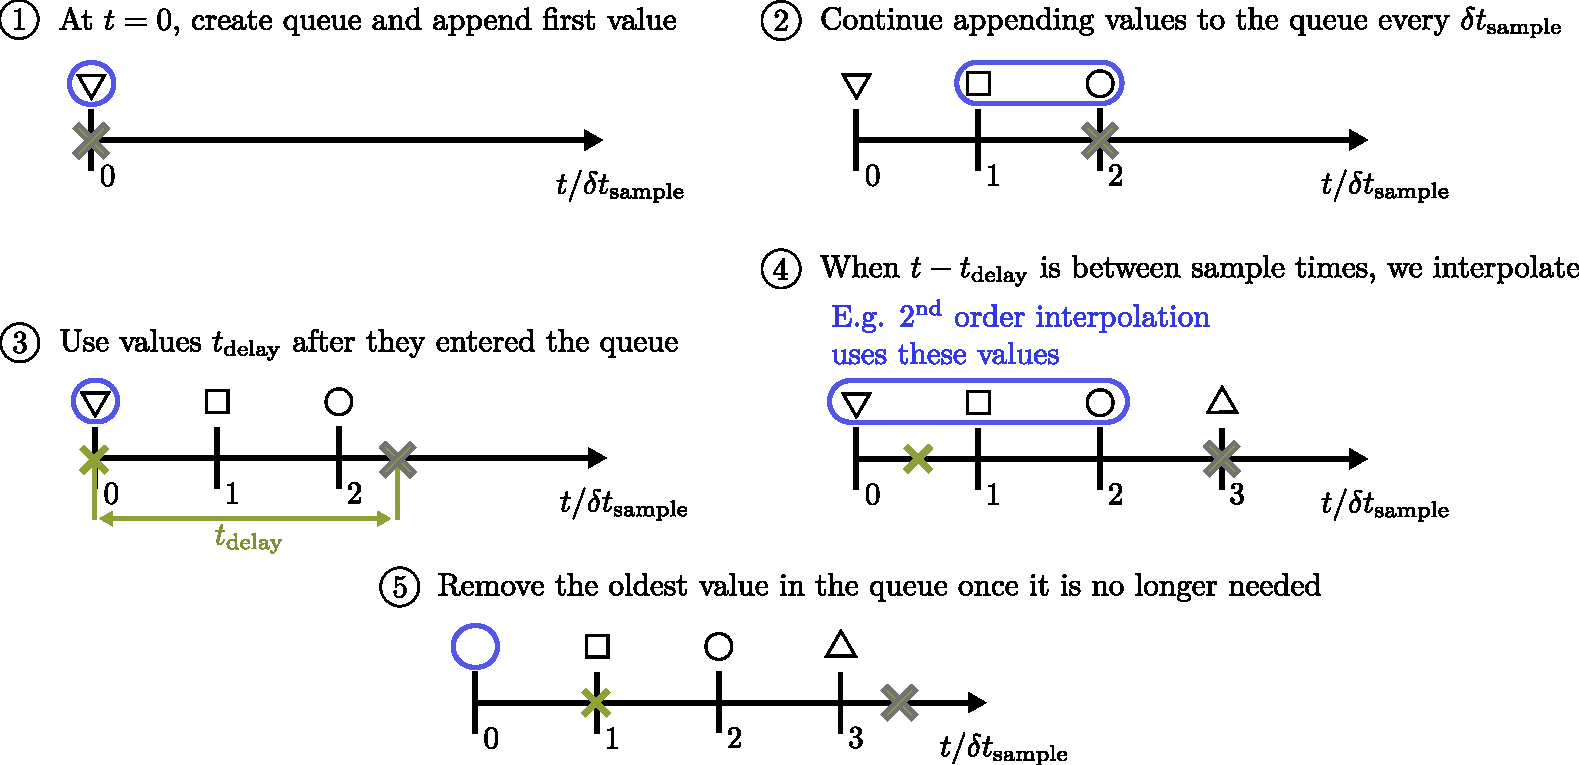
\includegraphics[scale=0.60]{assets/imgs/delay_bc_queue.pdf}
\caption{An illustration of how this queue system is used for boundary sampling. Different shapes are used to represent the different values in $\bb{T} \cross \bb{L}$. The values relevant to the current step is circled in blue.}
\label{fig:delay-queue}
\end{figure}

This queue system is illustrated in \fig{fig:delay-queue} in a continuous temporal domain for simplicity so sample times remain uniformly spaced. The first two steps, (1) and (2) show values being appended to the queue at the beginning of the simulation until the time delay is reached in the third step, (3). The fourth step, (4) shows which values are used in a second order interpolation. The final step, (5) shows old values being removed from the start of the queue.

\begin{figure}[t]
\centering
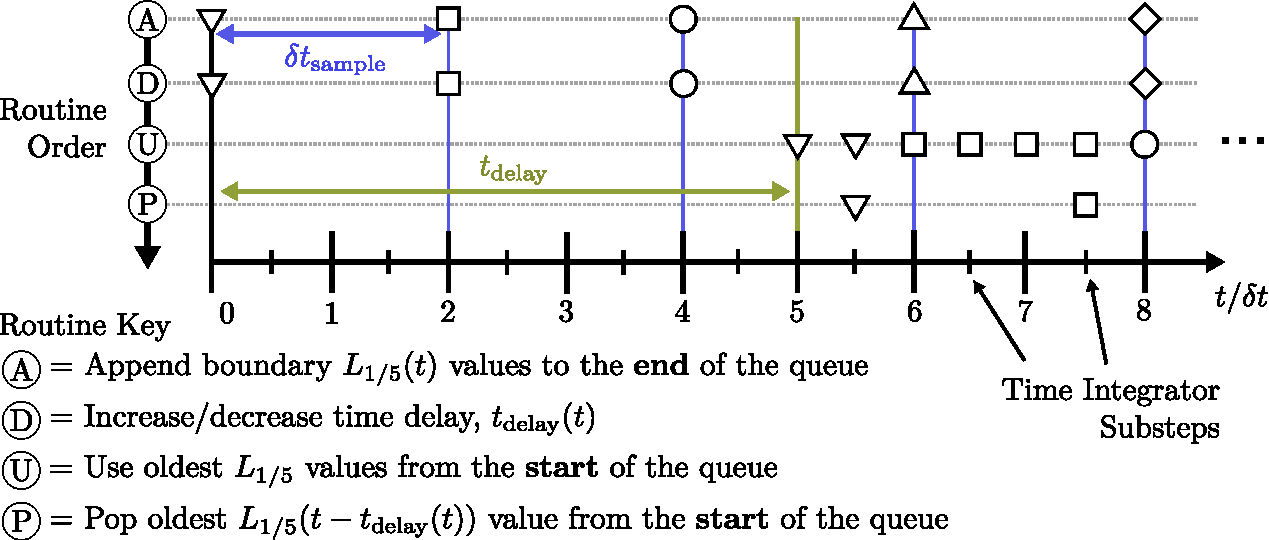
\includegraphics[scale=0.60]{assets/imgs/delay_bc_code_schematic.pdf}
\caption{Routine schematic for ADCBC implemented into a time integrator with two substeps. A sample period $δt_{\rm{sample}} = 2δt$ is used in this example. The evaluation of routines (or procedures) are shown in order from top to bottom (starting with (D) and ending with (U), key given in the figure), left to right (beginning at $t = 0$ and showing up to $t = 8 δt$). A routine being used is signified by a shape representing given sample in $\bb{T} \cross \bb{L}$. The time delay $τ \approx 4 \frac{3}{4} δt$ is shown in gold.}
\label{fig:schematic}
\end{figure}

As for an actual implementation into the multistep integration used in the SUNSET code, \fig{fig:schematic} illustrates the full schematic for a time integrator with two substeps per time step and uniform time step size. Sampling is performed in the routine (A) which is called every sample time preceded by a change to $τ$ in (D), if required. These are circled and labelled (1) and (2) corresponding to the steps in \fig{fig:delay-queue}. Only after the full time delay $τ$ do the values from the beginning of the queue get used for interpolation in the routine (U). This is illustrated in the labels (3) and (4) corresponding to those steps in \fig{fig:delay-queue}. Finally, step (5) removes the oldest value from the queue only once they are not needed in the routine (R). Appending and removal from the queue happen before the queue values are used for interpolation to ensure the correct values are available in the queue for interpolation. Note that the routine (U) happens every substep using as many values from the beginning of the queue as are required. The shape shown for this routine are just the earliest sample taken which would be used in steps (3) and (4).



\subsection{Memory Footprint}

The obvious disadvantage of this ADCBC method is the potential size of queues required to hold the data in $\bb{T} \cross \bb{L}$. This data should only be available to those processors relevant to the boundary nodes, so the memory burden should be held by those processors alone -- since the SUNSET code is run on distributed systems, where memory is allocated to each processor separately. If the memory footprint is too large (on the order of one gigabyte for modern hardware), then the simulations will likely crash and high-memory compute nodes would be required. Let us now perform a simple calculation to estimate the memory required by a given acoustic delay characteristic boundary. Assume $l = 1$ m, $c = 343$ m s$^{-1}$ and that a typical sample period is approximately $δt_{\rm{sample}} = 10^{-7}$ s (this will be validated in the coming chapter). Then, the number of numbers which need to be stored in memory are:
\begin{equation}
N_{\rm{numbers}} = 2 \frac{τ}{δt_{\rm{sample}}}
= \frac{4 \, l}{c \, δt_{\rm{sample}}}
\approx 1.17 \cross 10^5.
\end{equation}
For double precision floating point numbers, these require 8 bytes of storage each, resulting in $9.33 \cross 10^5$ bytes $\approx 1$ MB. This can easily be stored and accessed with modern memory, albeit may not be stored in the boundary processor's cache. Overall, this is not a concern as remaining memory required by the LABFM discretisation dwarfs this.

In an alternate formulation where acoustics across the boundary are not averaged and instead we have separate queues for samples taken at each boundary node, we are likely to have less than 100 boundary nodes per processor in two-dimensions (and fewer or the same in three). This results in a memory requirement lower than 100 MB, which is still manageable. If longer, e.g.\ $l = 10$ m, domains are modelled, then this would become a significant issue. Importantly, the total memory requirement under this method is significantly lower than if the fully nonlinear acoustics had been discretised in the up- and downstream regions, but these discretisations would be easier to decompose into separate processors. The potential issue then, comes from the fact that this memory burden is placed only onto the boundary nodes, which would have less memory available than the total memory provided in a theoretical decomposition of the acoustic region between more processors.



\section{Acoustic Region Field Reconstruction}

\begin{figure}[t]
\centering
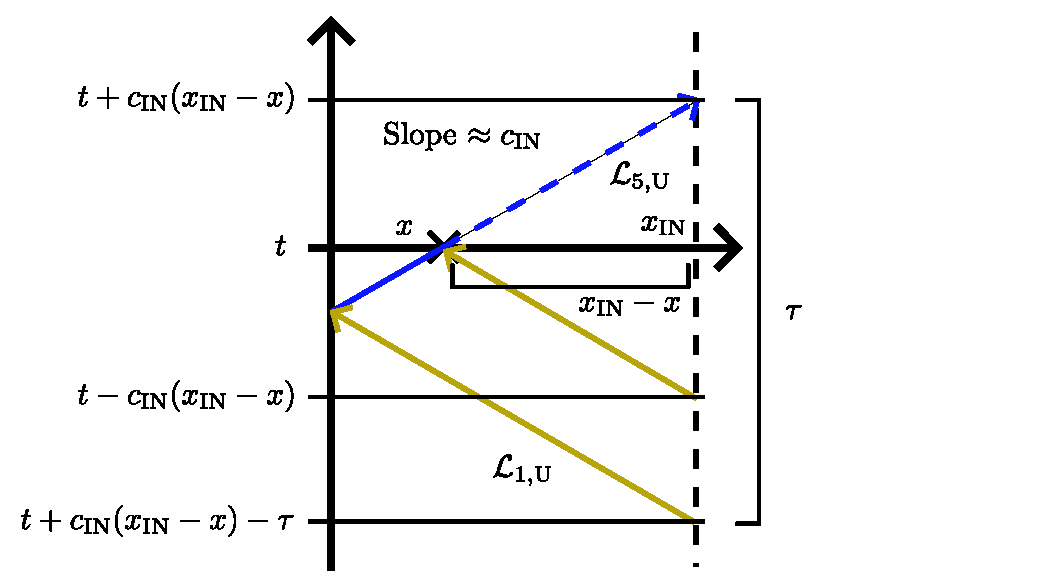
\includegraphics[scale=0.60]{assets/imgs/inlet-adcbc-spatial-field.pdf}
\caption{A simple diagram illustrating the time delays required to find $\cl{L}_{1/5, \rm{U}}(t, x)$ from a continuous field $\overline{\cl{L}}_{\rm{IN}}$ entering the upstream region at $x = x_{\rm{IN}}$.}
\label{fig:field-reconstruction}
\end{figure}

%%%%%% REWORD THIS FIRST SENTENCE !!!!
Already having made the low Mach and linear acoustics approximations makes the reconstruction of acoustic fields in an acoustic region simple as we can approximate the motion of acoustic variables $J_{1/5}$ through the acoustic region with a constant speed $c$. Hence, we can reinterpret a time series of previous $\overline{\cl{L}}_{\rm{IN/OUT}}(t')$ which leave the ADCBC boundaries as spatial information: the longer ago the acoustic exited through the ADCBC boundary, the farther into its acoustic trajectory it should be. Following the diagram shown in \fig{fig:field-reconstruction}, we have in the upstream region:
\begin{subequations}
\begin{alignat}{2}
\cl{L}_{1, \rm{U}}(t, x) &= &&\overline{\cl{L}}_{\rm{IN}}(t - c_{\rm{IN}}(x_{\rm{IN}} - x))
\quad \text{and} \\
\cl{L}_{5, \rm{U}}(t, x) &= R_{\rm{U}} \, &&\overline{\cl{L}}_{\rm{IN}}(t + c_{\rm{IN}}(x_{\rm{IN}} - x) - τ_{\rm{U}}),
\end{alignat}
and in the downstream region:
\begin{alignat}{2}
\cl{L}_{5, \rm{D}}(t, x) &= &&\overline{\cl{L}}_{\rm{OUT}}(t - c_{\rm{OUT}}(x - x_{\rm{OUT}}))
\quad \text{and} \\
\cl{L}_{1, \rm{D}}(t, x) &= R_{\rm{D}} \, &&\overline{\cl{L}}_{\rm{OUT}}(t + c_{\rm{OUT}}(x - x_{\rm{OUT}}) - τ_{\rm{D}}).
\end{alignat}
\end{subequations}
Using these fields, we can reconstruct the acoustic pressure and velocity by integrating backwards into the upstream region:
\begin{subequations}
\begin{alignat}{2}
p_{a, \rm{U}}(t, x) &= p_{a, \rm{U}}(t, x_{\rm{IN}}) + \frac{1}{2c_{\rm{IN}}} &&\int_{x}^{x_{\rm{IN}}} (\cl{L}_{1, \rm{U}}(t, x') - \cl{L}_{5, \rm{U}}(t, x')) \dd{x'}
\quad \text{and} \\
u_{a, \rm{U}}(t, x) &= u_{a, \rm{U}}(t, x_{\rm{IN}}) + \frac{1}{2c_{\rm{IN}}} \, \frac{1}{ρ_{\rm{IN}} c_{\rm{IN}}} &&\int_{x}^{x_{\rm{IN}}} (\cl{L}_{1, \rm{U}}(t, x') + \cl{L}_{5, \rm{U}}(t, x')) \dd{x'},
\end{alignat}
and forwards into the downstream region:
\begin{alignat}{2}
p_{a, \rm{D}}(t, x) &= p_{a, \rm{D}}(t, x_{\rm{OUT}}) + \frac{1}{2c_{\rm{OUT}}} &&\int_{x_{\rm{OUT}}}^{x} (\cl{L}_{5, \rm{D}}(t, x') - \cl{L}_{1, \rm{D}}(t, x')) \dd{x'}
\quad \text{and} \\
u_{a, \rm{D}}(t, x) &= u_{a, \rm{D}}(t, x_{\rm{OUT}}) + \frac{1}{2c_{\rm{OUT}}} \, \frac{1}{ρ_{\rm{OUT}} c_{\rm{OUT}}} &&\int_{x_{\rm{OUT}}}^{x} (\cl{L}_{1, \rm{D}}(t, x') + \cl{L}_{5, \rm{D}}(t, x')) \dd{x'}.
\end{alignat}
\end{subequations}
Notice that this means the upstream acoustic fields, for example, can be full reconstructed using information only from $t' \in [t - τ, t]$.

To use this continuous derivation with the discrete data, we must discretise the fields onto our samples $\bb{T}\cross\bb{L}$. This means defining the fields in the upstream upstream region as:
\begin{subequations}
\begin{alignat}{3}
\cl{L}_{1, \rm{U}}(t, x) &= &&\overline{\cl{L}}_{\rm{IN}, s_{1, \rm{U}}(t, x)}
\quad && \text{where} \quad
s_{1, \rm{U}}(t, x) \equiv \rm{round}(t - c_{\rm{IN}}(x_{\rm{IN}} - x))
\quad \text{and} \\
\cl{L}_{5, \rm{U}}(t, x) &= R_{\rm{U}} \, &&\overline{\cl{L}}_{\rm{IN}, s_{5, \rm{U}}(t, x)}
\quad && \text{where} \quad
s_{5, \rm{U}}(t, x) \equiv \rm{round}(t + c_{\rm{IN}}(x_{\rm{IN}} - x) - τ_{\rm{U}})
\end{alignat}
where the function round rounds to the nearest integer and in the downstream region:
\begin{alignat}{3}
\cl{L}_{5, \rm{D}}(t, x) &= &&\overline{\cl{L}}_{\rm{OUT}, s_{5, \rm{D}}(t, x)}
\quad && \text{where} \quad
s_{5, \rm{D}}(t, x) \equiv \rm{round}(t - c_{\rm{OUT}}(x - x_{\rm{OUT}}))
\quad \text{and} \\
\cl{L}_{1, \rm{D}}(t, x) &= R_{\rm{D}} \, &&\overline{\cl{L}}_{\rm{OUT}, s_{1, \rm{D}}(t, x)}
\quad && \text{where} \quad
s_{1, \rm{D}}(t, x) \equiv \rm{round}(t + c_{\rm{OUT}}(x - x_{\rm{OUT}}) - τ_{\rm{D}})
\end{alignat}
\end{subequations}
such that the discretised integrals become discrete sums:
\begin{subequations}
\begin{alignat}{2}
p_{a, \rm{U}}(t, x) &= p_{a, \rm{U}}(t, x_{\rm{IN}}) + \frac{1}{2} &&\left( \sum_{s = s_{1, \rm{U}}(t, x)}^{s_{1, \rm{U}}(t, x_{\rm{IN}})} \overline{\cl{L}}_{\rm{IN}, s} - \sum_{s = s_{5, \rm{U}}(t, x)}^{s_{5, \rm{U}}(t, x_{\rm{IN}})} \overline{\cl{L}}_{\rm{IN}, s} \right)δt_{\rm{sample}}
\quad \text{and} \\
u_{a, \rm{U}}(t, x) &= u_{a, \rm{U}}(t, x_{\rm{IN}}) + \frac{1}{2} \, \frac{1}{ρ_{\rm{IN}} c_{\rm{IN}}} &&\left( \sum_{s = s_{1, \rm{U}}(t, x)}^{s_{1, \rm{U}}(t, x_{\rm{IN}})} \overline{\cl{L}}_{\rm{IN}, s} + \sum_{s = s_{5, \rm{U}}(t, x)}^{s_{5, \rm{U}}(t, x_{\rm{IN}})} \overline{\cl{L}}_{\rm{IN}, s} \right) δt_{\rm{sample}}
\end{alignat}
and forwards into the downstream region:
\begin{alignat}{2}
p_{a, \rm{D}}(t, x) &= p_{a, \rm{D}}(t, x_{\rm{OUT}}) + \frac{1}{2} &&\left( \sum_{s = s_{5, \rm{D}}(t, x_{\rm{OUT}})}^{s_{5, \rm{D}}(t, x)} \overline{\cl{L}}_{\rm{OUT}, s} - \sum_{s = s_{1, \rm{D}}(t, x_{\rm{OUT}})}^{s_{1, \rm{D}}(t, x)} \overline{\cl{L}}_{\rm{OUT}, s} \right) δt_{\rm{sample}}
\quad \text{and} \\
u_{a, \rm{D}}(t, x) &= u_{a, \rm{D}}(t, x_{\rm{OUT}}) + \frac{1}{2} \, \frac{1}{ρ_{\rm{OUT}} c_{\rm{OUT}}} &&\left( \sum_{s = s_{1, \rm{D}}(t, x_{\rm{OUT}})}^{s_{1, \rm{D}}(t, x)} \overline{\cl{L}}_{\rm{OUT}, s} + \sum_{s = s_{5, \rm{D}}(t, x_{\rm{OUT}})}^{s_{5, \rm{D}}(t, x)} \overline{\cl{L}}_{\rm{OUT}, s} \right) δt_{\rm{sample}}
\end{alignat}
\end{subequations}
under the assumption that samples are equally spaced out such that $t_{s} - t_{s - 1} = δt_{\rm{sample}}$. For real simulation data from the SUNSET code variable time steps are used, so this assumption is impossible to enforce, which will introduce some error into the acoustic field reconstruction. Alternatively, we simply replace the sample spacing $δt_{\rm{sample}}$ by $t_{s} - t_{s - 1}$ in the sums above. In either case, these can be calculated from the sampled queue values $\bb{T}\cross\bb{L}$, which can be output from the SUNSET code at arbitrary times we want to observe the acoustic field. These fields can then be viewed using the above formulae as a post-processing step.




\section{Sampling Error}

\begin{figure}[t]
\centering
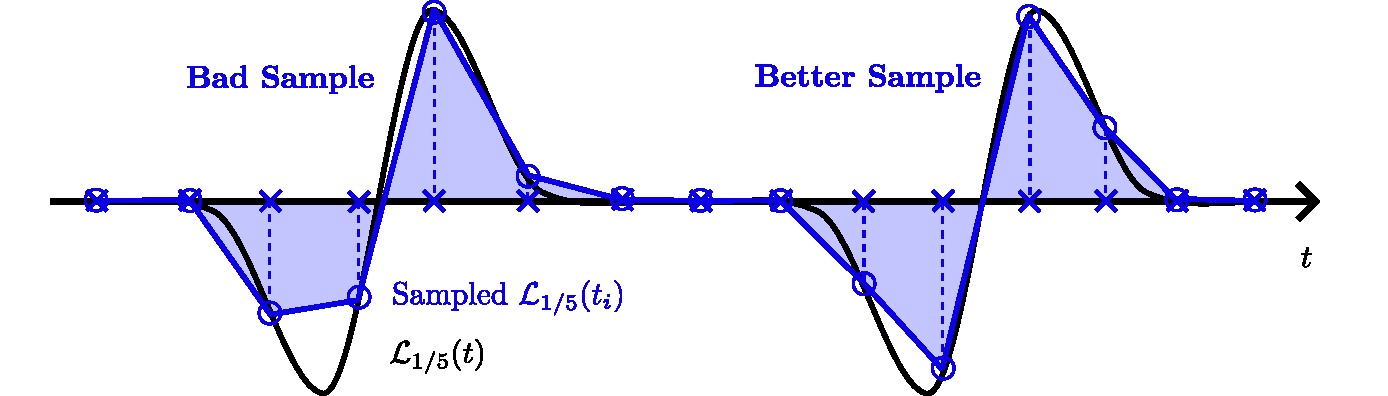
\includegraphics[scale=0.60]{assets/imgs/wave-sampling-comparison.pdf}
\caption{How ADCBCs might sample two Gaussian-shaped acoustic waves.}
\label{fig:wave-sampling}
\end{figure}

%%%%%% IS THERE A BETTER 
\fig{fig:wave-sampling} shows a representative analytic field $\cl{L}_{1, \rm{IN}}(t, y)$ for two acoustic bumps (which is roughly the derivative of a Gaussian). Despite a similar linear interpolation and sample period being used, the sampled $\overline{\cl{L}}_{1, s}$ values on the left are much worse than those on the right. The same could be true for any number of samples at a given interpolation order and sample period, where the change in phase and variability of the sampling will always cause some inaccuracy in the resulting integrated acoustic field upon reentry of these $\overline{\cl{L}}_{1, s}$ values. This inaccuracy results in a change to the shape of the disturbance which entered, e.g.\ a skew to one side, dissipation of acoustic energy or a drift in pressure and velocity behind the bump. These effects feed back into this issue at future reflections such that the waves eventually fully break down. Hence, small inaccuracies in integrated acoustic fields at reentry in the beginning of a simulation can result in large inaccuracies after more reflections. Note that the use of an acoustically conservative method for the ADCBCs would solve the issue of acoustic dissipation and pressure drift, but the destruction of the wave shape would remain. But, if the bump remains the same size and the tube is made longer, proportionally less reflections happen and the sampling error grows slower. If we begin with an error $\rm{err}_0$ which is amplified by $(1 + a)$ each reflection for some $a > 0$, then after $n$ reflections we have:
\begin{equation}
\rm{err}_A(n) \equiv (1 + a)^{n} \rm{err}_0.
\end{equation}
Thus, if the tube lengthens by a factor $b \equiv l_B / l_A > 1$, we instead expect to get only $n_B \equiv \lfloor n_A / b \rfloor$ reflections. This longer tube amplifies the error in the same way each reflection, so $\rm{err}_B(n) \equiv \rm{err}_A(n)$. Hence, the same number of reflections are required to reach the same error, or a time $t_B \approx b t_A$ to reach the same error. Considering this longer tube, we should acknowledge the longer associated wavelengths of acoustic will be sampled many more times, which we model by having each reflection amplify the error by a factor $(1 + a / b)$ instead. In this case:
\begin{equation}
\rm{err}_C(n) \equiv \left( 1 + \frac{a}{b} \right)^n \rm{err}_0,
\end{equation}
so $\rm{err}_C(n_C) = \rm{err}_B(n_B)$ if and only if $n_C \log(1 + a / b) = n_B \log(1 + a)$, or equivalently:
\begin{equation}
\frac{n_C}{n_B} = \frac{\log\left(1 + a\right)}{\log(1 + \frac{a}{b})} \xrightarrow{a \to 0^+} b
\end{equation}
so $b$ times more reflections are required to reach the same error or a time $t_C \approx b t_B$ in the asymptotic regime $a \ll 1$. Combined, these two effects result in a scaling of $t_C \approx b^2 t_A$. This quadratic scaling means that which are well-resolved by the ADCBCs in a short domain are very likely to be accurate in a long domain. Verifying the former, i.e.\ the usefulness of ADCBCs in short domains, is the premise of the the first two test cases in the coming chapter.



